

\begin{bt}{Ví dụ 1}
Giải hệ phương trình sau bằng phương pháp Newton-Raphson
\[
\begin{cases}
x^2 + y^2 - 4 = 0 & (1) \\
x^2 - y - 2 = 0 & (2)
\end{cases}
\]
Biết nghiệm chính xác của hệ là:$(x,y)=\{(\sqrt{3}, 1)$, $(-\sqrt{3}, 1)$, $(0, -2)\}$.

\end{bt}
{\textbf{Giải.}}

Phương pháp Newton-Raphson cho hệ nhiều biến sử dụng ma trận Jacobian ($J$). Công thức lặp có dạng:
\[
\begin{bmatrix}
x_{n+1} \\
y_{n+1}
\end{bmatrix}
= 
\begin{bmatrix}
x_n \\
y_n
\end{bmatrix}
- J^{-1}(x_n, y_n) \mathbf{F}(x_n, y_n)
\]

Ma trận Jacobian$J(x, y)$
\[
J(x, y) = 
\begin{bmatrix}
\dfrac{\partial f_1}{\partial x} & \dfrac{\partial f_1}{\partial y} \\[10pt]
\dfrac{\partial f_2}{\partial x} & \dfrac{\partial f_2}{\partial y}
\end{bmatrix}
= 
\begin{bmatrix}
2x & 2y \\
2x & -1
\end{bmatrix}
\]

Giả sử ta chọn điểm xuất phát gần nghiệm $(\sqrt{3}, 1) \approx (1.732, 1)$. Ta chọn $(x_0, y_0) = (1.5, 1.5)$.

Tính giá trị của hàm và Jacobian tại $(1.5, 1.5)$:
\[
\mathbf{F}(1.5, 1.5) = 
\begin{bmatrix}
1.5^2 + 1.5^2 - 4 \\
1.5^2 - 1.5 - 2
\end{bmatrix}
= 
\begin{bmatrix}
0.5 \\
-1.25
\end{bmatrix}
\]

\[
J(1.5, 1.5) = 
\begin{bmatrix}
3 & 3 \\
3 & -1
\end{bmatrix}
\]

Tính ma trận nghịch đảo $J^{-1}$:
\[
\det(J) = (3)(-1) - (3)(3) = -12
\]

\[
J^{-1} = \frac{1}{-12} 
\begin{bmatrix}
-1 & -3 \\
-3 & 3
\end{bmatrix}
\]

Cập nhật giá trị bước lặp tiếp theo $(x_1, y_1)$:
\[
\begin{bmatrix}
x_1 \\
y_1
\end{bmatrix}
= 
\begin{bmatrix}
1.5 \\
1.5
\end{bmatrix}
- \left( \frac{1}{-12} 
\begin{bmatrix}
-1 & -3 \\
-3 & 3
\end{bmatrix}
\right)
\begin{bmatrix}
0.5 \\
-1.25
\end{bmatrix}
\]

% \[
% \begin{bmatrix}
% x_1 \\
% y_1
% \end{bmatrix}
% = 
% \begin{bmatrix}
% 1.5 \\
% 1.5
% \end{bmatrix}
% + \frac{1}{12} 
% \begin{bmatrix}
% -1(0.5) - 3(-1.25) \\
% -3(0.5) + 3(-1.25)
% \end{bmatrix}
% \]
\[
\begin{bmatrix}
x_1 \\
y_1
\end{bmatrix}
= 
\begin{bmatrix}
1.5 \\
1.5
\end{bmatrix}
+ \frac{1}{12} 
\begin{bmatrix}
3.25 \\
-5.25
\end{bmatrix}
= 
\begin{bmatrix}
1.5 \\
1.5
\end{bmatrix}
+ 
\begin{bmatrix}
0.2708 \\
-0.4375
\end{bmatrix}
= 
\begin{bmatrix}
1.7708 \\
1.0625
\end{bmatrix}
\]

Thực hiện tương tự 4 lần lặp ta có bảng sau. 

\begin{table}[h]
\centering
\caption{Điểm bắt đầu $(1.5,1.5)$}

\begin{tabular}{|c|c|c|c|}
\hline
\textbf{$k$} & \textbf{$x_{1}^{(k)}$} & \textbf{$x_{2}^{(k)}$} & \textbf{$||x^{(k)} - x^{(k-1)}||_\infty$} \\
\hline
0 & 1.5000000000 & 1.5000000000 &  - \\
1 & 1.7708333333 & 1.0625000000 &  4.37500000e-01 \\
2 &1.7328284314 & 1.0012500000 &  6.12500000e-02 \\
3 &1.7320511322 & 1.0000005204 &  1.24947960e-03 \\
4 & 1.7320508076 & 1.0000000000 & 5.20399577e-07 \\
\hline
\end{tabular}
\end{table}

Cùng cách giải như vậy, nếu ta đổi điểm bắt đầu là $(2.0,2.0)$ và $(5.0,5.0)$
ta sẽ lần lượt được bảng như sau.


\begin{table}[h]
\centering
\caption{Điểm bắt đầu $(2,2)$}
\begin{tabular}{|c|c|c|c|}
\hline
\textbf{$k$} & \textbf{$x_{1}^{(k)}$} & \textbf{$x_{2}^{(k)}$} & \textbf{$||x^{(k)} - x^{(k-1)}||_\infty$} \\
\hline
0 & 2.0000000000 & 2.0000000000 &  - \\
1 &1.8000000000 & 1.2000000000 &8.00000000e-01 \\
2 &1.7366013072 & 1.0117647059 &1.88235294e-01 \\
3 &11.7320699496 & 1.0000457771 &1.17189288e-02 \\
4 & 1.7320508079 & 1.0000000007 &4.57763672e-05 \\
\hline
\end{tabular}    
\end{table}
\begin{table}[H]
\centering
\caption{Điểm bắt đầu $(5.0,5.0)$}
\begin{tabular}{|c|c|c|c|}
\hline
\textbf{$k$} & \textbf{$x_{1}^{(k)}$} & \textbf{$x_{2}^{(k)}$} & \textbf{$||x^{(k)} - x^{(k-1)}||_\infty$} \\
\hline
0 & 5.0000000000 & 5.0000000000 &  - \\
1 &2.9454545455 & 2.4545454545 &2.54545455e+00 \\
2 &2.0427652594 & 1.3580419580 &1.09650350e+00 \\
3 &1.7641251122 & 1.0344970799 &3.23544878e-01 \\
4 & 1.7324522887 & 1.0003877650 &3.41093149e-02 \\
\hline
\end{tabular}

\end{table}

Bằng mắt thường ta có thể thấy sai số phụ thuộc vào cách ta chọn điểm ban đầu. Khi chọn càng xa thì nó càng hội tụ chậm. Khi chọn càng gần nghiệm thì nó sẽ hội tụ nhanh hơn. 

Ngoài ra, nếu ta chọn điểm ban đầu là $(-2.0,5.0)$ thì ta sẽ có kết quả sau 4 lần lặp là bảng sau

\begin{table}[H]
\centering
\caption{Điểm bắt đầu $(-2.0,5.0)$}
\begin{tabular}{|c|c|c|c|}
\hline
\textbf{$k$} & \textbf{$x_{1}^{(k)}$} & \textbf{$x_{2}^{(k)}$} & \textbf{$||x^{(k)} - x^{(k-1)}||_\infty$} \\
\hline
0 & -2.0000000000 & 5.0000000000 &  - \\
1 &-2.1136363636 & 2.4545454545 &2.54545455e+00 \\
2 &-1.8511936988 & 1.3580419580 &1.09650350e+00 \\
3 &-1.7452023509 & 1.0344970799 &3.23544878e-01 \\
4 & -1.7322114560 & 1.0003877650 &3.41093149e-02 \\
\hline
\end{tabular}
\end{table}

Khi này dễ dàng nhận ra, việc lặp đã hội tụ về nghiệm $(-\sqrt3 ,1)$. 

Ngoài ra khi chọn $(0,0)$ làm điểm bắt đầu thì ta có được $J= \begin{bmatrix}
    0 &0\\0 &0
\end{bmatrix}$, hệ vô lý.

\subsubsection*{Kết luận rút ra}
 Kết quả hội tụ của hệ phương trình sẽ phụ thuộc vào cách mà ta chọn điểm ban đầu. Hơn nữa, nếu ta chọn chỉ 1 điểm bắt đầu thì kết quả trả ta cũng sẽ chỉ có 1 nghiệm trong khi nghiệm chính xác ta có tới 3 cặp thỏa mãn.\\
\begin{bt}{Ví dụ 2}
Giải hệ phương trình phi tuyến sau:
\begin{align*}
    3x_{1} - \cos(x_{2}x_{3}) - \frac{1}{2} &= 0 \\
    x_{1}^{2} - 81(x_{2} + 0.1)^{2} + \sin x_{3} + 1.06 &= 0 \\
    e^{-x_{1}x_{2}} + 20x_{3} + \frac{10\pi - 3}{3} &= 0
\end{align*}
với giá trị ban đầu là
\[
x^{(0)} = \begin{bmatrix} 0.1 \\ 0.1 \\ -0.1 \end{bmatrix}
\]
\end{bt}
\textbf{Giải.}

Ta có vector ban đầu
\[
x^{(0)} = \begin{bmatrix} 0.1 \\ 0.1 \\ -0.1 \end{bmatrix}
\]

Lại có
\[
F(x) = \begin{bmatrix}
3x_{1} - \cos(x_{2}x_{3}) - \frac{1}{2} \\
x_{1}^{2} - 81(x_{2} + 0.1)^{2} + \sin x_{3} + 1.06 \\
e^{-x_{1}x_{2}} + 20x_{3} + \frac{10\pi - 3}{3}
\end{bmatrix}
\]
\[
J(x) = \begin{bmatrix}
3 & x_{3}\sin(x_{2}x_{3}) & x_{2}\sin(x_{2}x_{3}) \\
2x_{1} & -162(x_{2} + 0.1) & \cos x_{3} \\
-x_{2}e^{-x_{1}x_{2}} & -x_{1}e^{-x_{1}x_{2}} & 20
\end{bmatrix}
\]

Tiếp theo ta cần tính $F(x^{(0)})$ và $J(x^{(0)})$ với $x^{(0)} = (0.1, 0.1, -0.1)^{T}$:
\[
F(x^{(0)}) 
%= 
% \begin{bmatrix}
% 0.3 - \cos(-0.01) - \frac{1}{2} \\
% 0.01 - 3.24 + \sin(-0.1) + 1.06 \\
% e^{(-0.01)} - 2 + \frac{10\pi - 3}{3}
% \end{bmatrix}
= \begin{bmatrix}
-1.19995 \\
-2.269833417 \\
8.462025346
\end{bmatrix}
\]
và
\begin{align*}
J(x^{(0)}) 
% &= \begin{bmatrix}
% 3 & (-0.1)\sin(-0.01) & 0.1\sin(-0.01) \\
% 0.2 & -162(0.2) & \cos(-0.1) \\
% -0.1e^{-0.01} & -0.1e^{-0.01} & 20
% \end{bmatrix} \\
&= \begin{bmatrix}
3 & 0.000999983 & -0.000999983 \\
0.2 & -32.4 & 0.995004165 \\
-0.099004984 & -0.099004983 & 20
\end{bmatrix}
\end{align*}

Giải hệ $J(x^{(0)})y^{(0)} = -F(x^{(0)})$ tương đương:
\[
\begin{bmatrix}
3 & 0.000999983 & -0.000999983 \\
0.2 & -32.4 & 0.995004165 \\
-0.099004984 & -0.099004983 & 20
\end{bmatrix}
\begin{bmatrix} y_{1}^{(0)} \\ y_{2}^{(0)} \\ y_{3}^{(0)} \end{bmatrix}
= \begin{bmatrix}
1.19995 \\
2.269833417 \\
-8.462025346
\end{bmatrix}
\]
Sau khi giải hệ phương trình tuyến tính trên, ta thu được kết quả:
\[
y^{(0)} = \begin{bmatrix}
0.399867629 \\
-0.074369708 \\
-0.421489971
\end{bmatrix}
\]

Tính $x^{(1)} = x^{(0)} + y^{(0)}$:
\[
x^{(1)} = \begin{bmatrix} 0.1 \\ 0.1 \\ -0.1 \end{bmatrix} + \begin{bmatrix} 0.399867629 \\
-0.074369708 \\
-0.421489971 \end{bmatrix}
= \begin{bmatrix} 0.4998696729 \\ 0.0256303292 \\ -0.521489971\end{bmatrix}
\]
Ta có thể sử dụng kết quả của $x^{(1)}$ để tìm bước lặp tiếp theo $x^{(2)}$ bằng quy trình tương tự.

Nếu tiếp tục lặp lại quá trình này, ta sẽ nhận được các kết quả sau:

\begin{table}[h]
\centering
\begin{tabular}{|c|c|c|c|c|}
\hline
\textbf{$k$} & \textbf{$x_{1}^{(k)}$} & \textbf{$x_{2}^{(k)}$} & \textbf{$x_{3}^{(k)}$} & \textbf{$||x^{(k)} - x^{(k-1)}||_\infty$} \\
\hline
0 & 0.10000000 & 0.10000000 & -0.10000000 & - \\
1 & 0.4998696729 & 0.0256303292 & -0.5215204719 & 4.21520472e-01 \\
2 & 0.5000142402 & 0.0015885914 & -0.5235569643 &1.78782572e-02 \\
3 & 0.5000001135 & 0.0000124448 & -0.5235984501 &1.57614659e-03 \\
4 & 0.5000000000 & 0.0000000008 & -0.5235987756 &1.24440075e-05 \\
5 & 0.5000000000 & 0.0000000000 & -0.5235987756 &7.75785713e-10 \\
\hline
\end{tabular}
\end{table}

Ta biết rằng khi một tập hợp các vector hội tụ thì chuẩn $||x^{(k)} - x^{(k-1)}|| = 0$.

Do đó, theo bảng trên, chuẩn bằng 0 ở bước lặp thứ năm. Điều này cho thấy hệ $F(x)$ của chúng ta đã hội tụ về nghiệm, được ký hiệu là $\overline{x}$.

Vì vậy, từ bảng kết quả, ta biết rằng
\[
\overline{x} = \begin{bmatrix} 0.5000000 \\ 0.0000000 \\ -0.52359877 \end{bmatrix}
\]

% là một nghiệm xấp xỉ của $F(x) = 0$.

\begin{bt}{Ví dụ}
Ứng dụng phương pháp Newton-Raphson xác định điểm làm việc tĩnh $(Voltage,\ Current)$ của diode trong mạch, biết biểu thức xác định dòng điện qua mạch là $I_D = I_S \left( e^{\frac{V_D}{V_T}} - 1 \right)
$. Và Thông số Diode (mô hình lý tưởng):
    \begin{itemize}[label=\textbullet]
    \item Dòng bão hòa ngược: $I_S = 10^{-12} \, A$
    \item Điện áp nhiệt (ở nhiệt độ phòng): $V_T = 0.026V$
    \item Hệ số lý tưởng: $\eta = 1$
    \end{itemize}
\begin{figure}[H]
    \centering
    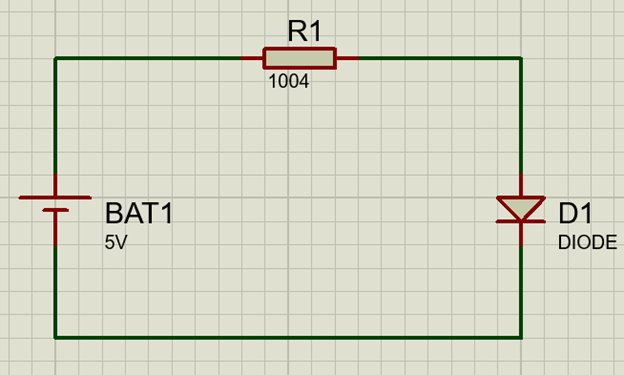
\includegraphics[width=0.5\textwidth]{pic/Ảnh PPT 1.png}
    \label{fig:hinh1}
\end{figure}
\end{bt}

{\textbf{Giải.}}
Áp dụng định luật Kirchhoff về điện áp (KVL) cho vòng kín, ta có phương trình:
\begin{equation}
E - I_D R - V_D = 0
\end{equation}

Thay phương trình Shockley:
\begin{equation}
I_D = I_S \left( e^{\frac{V_D}{V_T}} - 1 \right)
\end{equation}
vào KVL, ta xây dựng được hàm $f(V_D)$ cần tìm nghiệm:
\begin{equation}
f(V_D) = 5 - 1004 \cdot 10^{-12} \left( e^{\frac{V_D}{0.026}} - 1 \right) - V_D = 0
\end{equation}

Để áp dụng Newton-Raphson, ta cần đạo hàm bậc nhất của hàm số trên theo $V_D$ (đây chính là Jacobian 1 chiều của mạch):
\begin{equation}
f'(V_D) = -1 - \frac{1004 \cdot 10^{-12}}{0.026} e^{\frac{V_D}{0.026}}
\end{equation}

Công thức lặp Newton-Raphson cho mạch này sẽ là:
\begin{equation}
V_D^{(k+1)} = V_D^{(k)} - \frac{f(V_D^{(k)})}{f'(V_D^{(k)})}
\end{equation}

\subsubsection*{Kết quả}
\noindent \textbf{--} Sử dụng chương trình đã viết ở phần trước, ta chọn giá trị đoán nhận ban đầu cho điện áp Diode là $V_0 = 0.6V$ (đây là mức điện áp phân cực thuận thông thường của Diode Silicon để tránh thuật toán bị tràn số).\\ \noindent \textbf{--} Bảng kết quả ghi nhận sau mỗi vòng lặp:

\begin{table}[h]
\centering
\begin{tabular}{|c|c|c|c|c|}
    \renewcommand{\arraystretch}{1.2} % Tăng độ rộng giữa các hàng một chút cho dễ nhìn
        Lần lặp ($k$) & $V_D$ (V) & $f(V_D)$ (V) &$\Delta V$ (V) \\
        \hline
        0 & 0.6000000000 & -6.1660841311 & - \\
        \hline
        1 & 0.5848643397 & -1.4881464157  & 1.51356603e-02 \\
        \hline
        2 & 0.5783387930 & -0.1713043894  & 6.52554664e-03 \\
        \hline
        3 & 0.5773745264 & -0.0031200224  & 9.64266616e-04 \\
        \hline
        4 & 0.5773563042 & -0.0000010861  & 1.82222261e-05 \\
        \hline
        5 & 0.5773562979 & -0.0000000082  & 6.35121443e-09 \\
        \hline
\end{tabular}
\end{table}


\begin{itemize}[label=\textbf{+}]
    \item \textbf{Điểm làm việc tĩnh:} $Q=(V_D,I_D) \approx (0.577V,4.4mA)$.
    \item \textbf{Tốc độ hội tụ:} Nhìn vào bảng kết quả, ta thấy thuật toán tiến tới nghiệm chính xác chỉ sau đúng 5 lần lặp. Ở lần lặp thứ 5, sai số $\Delta V$ đã tiến sát về 0, chứng minh tính hội tụ cực kỳ mạnh mẽ của phương pháp Newton-Raphson. 
\end{itemize}
\subsubsection*{Đối chiếu với kết quả tính toán và thực tế}
\noindent \textbf{--} Để đánh giá độ chính xác của chương trình giải tích bằng thuật toán Newton-Raphson, ta tiến hành so sánh nghiệm điện áp $V_D$ tìm được với kết quả đo lường từ mô phỏng PROTEUS (phần mềm chuẩn công nghiệp) và các yếu tố trong thực nghiệm đo lường vật lý.
\begin{table}[h]
    \centering
    \renewcommand{\arraystretch}{1.5}
    % Thêm lệnh ép căn trái cho 3 cột X
    \begin{tabularx}{\textwidth}{|l|>{\raggedright\arraybackslash}X|>{\raggedright\arraybackslash}X|>{\raggedright\arraybackslash}X|}
        \hline
        \textbf{Thông số} & \textbf{Kết quả từ code Newton-Raphson} & \textbf{Kết quả mô phỏng PROTEUS} & \textbf{Đo lường thực tế Diode 1N4148 } \\
        \hline
        Điện áp Diode ($V_D$) & 0.577 V & $\sim$ 0.577 V & $\sim$ 0.620 V - 0.650 V \\
        \hline
        Dòng điện ($I_D$) & 4.40 mA & $\sim$ 4.40 mA & $\sim$ 4.35 mA \\
        \hline
        Thời gian giải & Vài mili-giây (4 vòng lặp) & Tương đương & N/A \\
        \hline
    \end{tabularx}
\end{table}
\\
\\
\noindent \textbf{--} Từ bảng số liệu trên, ta rút ra các kết luận quan trọng sau:
\begin{itemize}[label=\textbf{+}]
    \item \textbf{Sự chính xác về mặt toán học: } Kết quả từ chương trình code tự viết hoàn toàn trùng khớp với kết quả từ phần mềm mô phỏng PROTEUS khi sử dụng cùng một bộ thông số lý tưởng ($I_S = 10^{-12} \, A$, $n = 1$). Điều này khẳng định thuật toán Newton-Raphson và ma trận Jacobian thiết lập hoàn toàn chính xác.
    \item \textbf{Sự sai lệch so với linh kiện thực tế:} Khi đo trên mạch vật lý với một Diode thực tế (như 1N4148), điện áp VD thường lớn hơn kết quả tính toán (khoảng $0.62V - 0.65V$ so với $0.577V$). Sự chênh lệch này không phải do lỗi thuật toán, mà do mô hình toán học chưa bao quát hết các yếu tố vật lý thực tế. 
\end{itemize}

\noindent \textbf{--} Tuy nhiên nếu ta muốn code của chúng ta có thể thực hiện ra kết quả sát thực tế (thứ mà ta sử dụng phần mềm đo được), ta có thể cần đến vài điều kiện được lấy trong Datasheet của linh kiện và các thực nghiệm:

\begin{itemize}
    \item Hệ số lý tưởng $n=1.9$ 
    \item Dòng rò thực tế đo được $I_s\approx 4.35.10^{-9} A$
    \item Nội trở của Diode $R_S\approx 1 \Omega $ 
\end{itemize}

\noindent \textbf{--} Khi này thì ta có điện áp rơi trên Diode $V_{measured} = I_D.R_S + V_D$

Tính toán ta có 
\begin{equation}
    f(V_D) =  I_S \cdot e^{\frac{V_D}{n V_T}} + \frac{V_D - E}{R} = 0
\end{equation}

Đạo hàm Jacobian 

\begin{equation}
    f'(V_D) = \frac{I_S}{n V_T} e^{\frac{V_D}{n V_T}} + \frac{1}{R}
\end{equation}

Khi này ta giải như việc ta giải phương trình phi tuyến bình thường và sau khi chọn $V_D = 0,6 V$ thì ta tìm được giá trị $V_D$ sau 4 lần lặp là $0.6819V$, lúc này ta cộng thêm phần rơi áp nội trở nữa thì ta có được $V_{measured} = 0.682$ cũng xem như gần bằng giá trị đo được trong Proteus 
% \begin{bt}{Ví dụ}
% Ứng dụng phương pháp Newton-Raphson xác định điểm làm việc tĩnh (Q-point) của mạch gồm 2 Diode
% \end{bt}

% \subsubsection*{Sơ đồ và thông số mạch}
% \noindent \textbf{--} Xét mạch điện có 2 nút điện áp $V_1$ và $V_2$ chưa biết, bao gồm:
% \begin{itemize}[label=\textbf{+}]
%     \item Nguồn áp DC: $E = 10V$
%     \item Điện trở: $R_1 = 1000 \, \Omega, R_2 = 500 \, \Omega$
%     \item Hai Diode giống hệt nhau: $I_S = 10^{-12}A, V_T = 0.026V, n = 1$.
% \end{itemize}
% \noindent \textbf{--} Cấu trúc mạch:
% \begin{figure}[H]
%     \centering
%     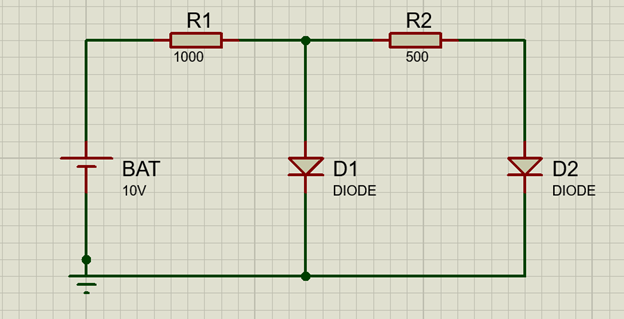
\includegraphics[width=0.8\textwidth]{pic/Ảnh PPT 2.png}
%     \caption{Cấu trúc mạch 2 diode (vẽ bằng Proteus)}
%     \label{fig:hinh1}
% \end{figure}
% \textcolor{blue}{\textbf{Giải.}}
% \subsubsection*{Thiết lập phương trình}
% \noindent \textbf{--} Gọi $V_1$ và $V_2$ lần lượt là điện áp tại Nút 1 và Nút 2. Áp dụng định luật KCL (tổng dòng điện rời khỏi nút bằng 0), ta có hệ phương trình:
% \begin{itemize}[label=\textbf{+}]
%     \item \textbf{Tại Nút 1: }Dòng qua $R_1$ + dòng qua $R_2$ + dòng qua $D_1$ = 0 \\
%     \\
%     $\frac{V_1 - E}{R_1} + \frac{V_1 - V_2}{R_2} + I_S \left( e^{\frac{V_1}{V_T}} - 1 \right) = 0$
%     \item \textbf{Tại Nút 2:}Dòng qua $R_2$ (từ 2 về 1) + dòng qua $D_2$ = 0
%     \\
%     \\
%     $\frac{V_2 - V_1}{R_2} + I_S \left( e^{\frac{V_2}{V_T}} - 1 \right) = 0$
% \end{itemize}

% Vector hàm số: $\mathbf{F}(\mathbf{V}) = \begin{bmatrix} f_1(V_1, V_2) \\ f_2(V_1, V_2) \end{bmatrix} = \mathbf{0}$

% \subsubsection*{Thiết lập ma trận Jacobian}
% \noindent \textbf{--} Để giải hệ này bằng Newton-Raphson, ta phải tính ma trận đạo hàm riêng (Jacobian matrix) kích thước  $2 \times 2$:
% \begin{equation}
% \mathbf{J}(V_1, V_2) = \begin{bmatrix} 
% \frac{\partial f_1}{\partial V_1} & \frac{\partial f_1}{\partial V_2} \\ 
% \frac{\partial f_2}{\partial V_1} & \frac{\partial f_2}{\partial V_2} 
% \end{bmatrix}
% \end{equation}

% \noindent \textbf{--}Chi tiết các đạo hàm:
% \begin{itemize}[label=\textbf{+}]
%     \item $\frac{\partial f_1}{\partial V_1} = \frac{1}{R_1} + \frac{1}{R_2} + \frac{I_S}{V_T} e^{\frac{V_1}{V_T}}$
%     \item $\frac{\partial f_1}{\partial V_2} = -\frac{1}{R_2}$
%     \item $\frac{\partial f_2}{\partial V_1} = -\frac{1}{R_2}$
%     \item $\frac{\partial f_2}{\partial V_2} = \frac{1}{R_2} + \frac{I_S}{V_T} e^{\frac{V_2}{V_T}}$
% \end{itemize}

% \subsubsection*{Biểu thức lặp ma trận}
% \hspace{0.4cm}Công thức lặp Newton-Raphson bây giờ sẽ làm việc trên vector thay vì số vô hướng:
% \begin{equation}
% \begin{bmatrix} V_1^{(k+1)} \\ V_2^{(k+1)} \end{bmatrix} = \begin{bmatrix} V_1^{(k)} \\ V_2^{(k)} \end{bmatrix} - \mathbf{J}^{-1} \cdot \begin{bmatrix} f_1(V_1^{(k)}, V_2^{(k)}) \\ f_2(V_1^{(k)}, V_2^{(k)}) \end{bmatrix}
% \end{equation}

% \subsubsection*{Kết quả}
% \begin{table}[H]
%     \centering
%     \small % Thu nhỏ font chữ để bảng gọn hơn
%     \setlength{\tabcolsep}{3pt} % Giảm khoảng cách giữa các cột (mặc định là 6pt)
%     \renewcommand{\arraystretch}{1.5}
    
%     % Cột 1 là 'c' (căn giữa theo nội dung), 6 cột còn lại là 'X' (tự động chia đều)
%     \begin{tabularx}{\textwidth}{|c|>{\centering\arraybackslash}X|>{\centering\arraybackslash}X|>{\centering\arraybackslash}X|>{\centering\arraybackslash}X|>{\centering\arraybackslash}X|>{\centering\arraybackslash}X|}
%         \hline
%         \textbf{$k$} & \textbf{$V_1$ (V)} & \textbf{$V_2$ (V)} & \textbf{Hàm KCL Nút 1 $f_1$ (A)} & \textbf{Hàm KCL Nút 2 $f_2$ (A)} & \textbf{Bước nhảy $\Delta V_1$ (V)} & \textbf{Bước nhảy $\Delta V_2$ (V)} \\
%         \hline
%         0 & 0.600000 & 0.600000 & $1.100 \times 10^{-3}$ & $1.050 \times 10^{-2}$ & -0.002845 & -0.025801 \\
%         \hline
%         1 & 0.597155 & 0.574199 & $1.254 \times 10^{-4}$ & $3.851 \times 10^{-3}$ & -0.000614 & -0.043175 \\
%         \hline
%         2 & 0.596541 & 0.531024 & $8.520 \times 10^{-6}$ & $7.412 \times 10^{-4}$ & -0.000051 & -0.027609 \\
%         \hline
%         3 & 0.596490 & 0.503415 & $1.140 \times 10^{-7}$ & $8.230 \times 10^{-5}$ & -0.000001 & -0.004805 \\
%         \hline
%         4 & 0.596489 & 0.498610 & $2.051 \times 10^{-10}$ & $2.140 \times 10^{-6}$ & 0.000000 & -0.000088 \\
%         \hline
%         5 & 0.596489 & 0.498522 & 0 & $1.420 \times 10^{-9}$ & 0.000000 & 0.000000 \\
%         \hline
%     \end{tabularx}
% \end{table}
% \noindent \textbf{--} \textbf{Điểm làm việc tĩnh (Q-Point):}
% \begin{itemize}[label=\textbf{+}]
%     \item Điện áp Nút 1: $V_1 \approx 0.5965 \, V$ (đây cũng là điện áp rơi trên Diode 1)
%     \item Điện áp Nút 2: $V_2 \approx 0.4985 \, V$ (đây cũng là điện áp rơi trên Diode 2)
% \end{itemize}
% \noindent \textbf{--} \textbf{Phân bố dòng điện:}
% \begin{itemize}[label=\textbf{+}]
%     \item Dòng tổng từ nguồn cấp (qua $R_1$): \[
%     I_{R1} = \frac{E - V_1}{R_1} = \frac{10 - 0.5965}{1000} \approx 9.403 \text{ mA}
% \]
%     \item Dòng điện qua Diode 1: \[
%     I_{D1} = 10^{-12} \left( e^{\frac{0.5965}{0.026}} - 1 \right) \approx 9.206 \text{ mA}
% \]
%     \item Dòng điện qua điện trở $R_2$ và Diode 2: \[
%     I_{D2} = I_{R2} = \frac{V_1 - V_2}{R_2} = \frac{0.5965 - 0.4985}{500} \approx 0.196 \text{ mA}
% \]
% \end{itemize}
% \noindent \textbf{--} \textbf{Đánh giá kết quả hội tụ:}
% \begin{itemize}[label=\textbf{+}]
%     \item Thuật toán hội tụ hoàn toàn ở vòng lặp thứ 5. Tại đây, giá trị hàm $f_1$ và $f_2$ (đại diện cho phần dư dòng điện tại các nút) đã tiến cực kỳ sát về 0 (đạt mức nano-Ampe). Điều này chứng tỏ định luật Kirchhoff (KCL) đã được thỏa mãn tuyệt đối.
%     \item Bước nhảy của điện áp ($\Delta V_1$ và $\Delta V_2$) cũng triệt tiêu về 0, chứng tỏ điểm làm việc tĩnh đã được chốt và không còn dao động.
% \end{itemize}
% \noindent \textbf{--} \textbf{Nhận xét về mặt kỹ thuật:}\begin{itemize}[label=\textbf{}]
%     \item Tại sao $V_1$ lại lớn hơn hẳn $V_2$ (0.596V so với 0.498V)?
% \end{itemize}
% $\Rightarrow$ Bởi vì Diode 1 nối trực tiếp vào Nút 1 nên nó gánh gần như toàn bộ dòng điện từ nguồn đổ về (hơn 9.2 mA). Trong khi đó, dòng điện muốn đến được Diode 2 phải đi qua điện trở $R_2$ (500 $\Omega$), gây ra hiện tượng sụt áp. Do dòng qua Diode 2 rất nhỏ (chỉ khoảng 0.2 mA), nên điện áp phân cực thuận của nó cũng thấp hơn nhiều theo đúng hàm logarit của đặc tuyến Diode.
% \subsubsection*{Đối chiếu với kết quả tính toán và thực tế}
% \begin{table}[h]
%     \centering
%     \renewcommand{\arraystretch}{1.5}
%     \begin{tabularx}{\textwidth}{|l|>{\raggedright\arraybackslash}X|>{\raggedright\arraybackslash}X|>{\raggedright\arraybackslash}X|}
%         \hline
%         \textbf{Thông số / Biến trạng thái} & \textbf{Code Newton-Raphson (Lý thuyết $n=1$)} & \textbf{Mô phỏng PROTEUS (Diode lý tưởng)} & \textbf{Đo lường thực tế (Sử dụng 2 Diode 1N4148)} \\
%         \hline
%         Điện áp Nút 1 ($V_1$) & 0.5965 V & 0.5965 V & $\approx$ 0.645 V \\
%         \hline
%         Điện áp Nút 2 ($V_2$) & 0.4985 V & 0.4985 V & $\approx$ 0.530 V \\
%         \hline
%         Dòng qua Diode 1 ($I_{D1}$) & 9.206 mA & 9.206 mA & $\approx$ 9.05 mA \\
%         \hline
%         Dòng qua Diode 2 ($I_{D2}$) & 0.196 mA & 0.196 mA & $\approx$ 0.22 mA \\
%         \hline
%     \end{tabularx}
% \end{table}
% \noindent \textbf{--} Từ bảng số liệu trên, ta rút ra các kết luận quan trọng sau:
% \begin{itemize}[label=\textbf{+}]
%     \item \textbf{Độ tin cậy của thuật toán:} Sự trùng khớp tuyệt đối (đến chữ số thập phân thứ 4) giữa chương trình tự viết và phần mềm PROTEUS chứng minh rằng hệ phương trình giải tích KCL và ma trận đạo hàm Jacobian 2 x 2 đã được thiết lập và lập trình hoàn toàn chính xác
%     \item \textbf{Sự khác biệt so với thực tế:} Do ta giả định hai Diode $D_1$ và $D_2$ giống hệt nhau (cùng $I_S$, cùng $n$). Tuy nhiên, trong thực tế chế tạo bán dẫn, không có hai linh kiện nào giống nhau 100\%. Thông số $I_S$ của $D_1$ và $D_2$ đo đạc thực tế có thể lệch nhau từ 5\% đến 10\%. Điều này làm sai lệch hệ phương trình.
% \end{itemize}
\begin{bt}{Ví dụ}
Ứng dụng phương pháp Newton-Raphson xác định điểm làm việc tĩnh $(Voltage,\ Current)$ của diode trong mạch, biết biểu thức xác định dòng điện qua mạch là $I_D = I_S \left( e^{\frac{V_D}{V_T}} - 1 \right)
$. Và Thông số Diode (mô hình lý tưởng):
    \begin{itemize}[label=\textbullet]
    \item Dòng bão hòa ngược: $I_S = 4.35 \cdot 10^{-9} \, A$
    \item Điện áp nhiệt (ở nhiệt độ phòng): $V_T = 0.026V$
    \item Hệ số lý tưởng: $\eta = 1.9$
    \item Giá trị mẫu số mũ: $n \cdot V_T = 1.9 \cdot 0.026 = 0.0494 V$
    \end{itemize}
    
    
\begin{figure}[H]
    \centering
    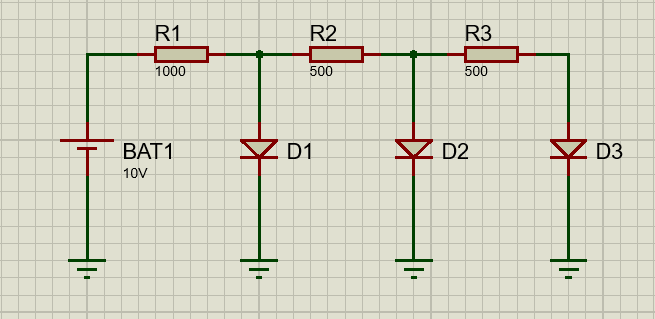
\includegraphics[width=0.5\textwidth]{pic/D3.png}
    \caption{Cấu trúc mạch 3 diode (vẽ bằng Proteus)}
    \label{fig:hinh1}
\end{figure}\end{bt}
\subsubsection*{Sơ đồ và thông số mạch}
{\textbf{Giải.}}
 Áp dụng định luật KCL tại 3 nút, ta thiết lập hệ phương trình phi tuyến dựa trên dòng điện qua diode $I_D = I_S(e^{\frac{V_D}{V_T}} - 1)$:
\begin{itemize}[label=\textbf{+}]
    \item \textbf{Tại Nút 1:} $\frac{V_1 - E}{R_1} + \frac{V_1 - V_2}{R_2} + I_S(e^{\frac{V_1}{n V_T}} - 1) = 0$ \\[8pt]
    $\Leftrightarrow \frac{V_1 - 10}{1000} + \frac{V_1 - V_2}{500} + 4.35 \cdot 10^{-9} \left( e^{\frac{V_1}{0.0494}} - 1 \right) = 0$
    
    \item \textbf{Tại Nút 2:} $\frac{V_2 - V_1}{R_2} + \frac{V_2 - V_3}{R_3} + I_S(e^{\frac{V_2}{n V_T}} - 1) = 0$ \\[8pt]
    $\Leftrightarrow \frac{V_2 - V_1}{500} + \frac{V_2 - V_3}{500} + 4.35 \cdot 10^{-9} \left( e^{\frac{V_2}{0.0494}} - 1 \right) = 0$
    
    \item \textbf{Tại Nút 3:} $\frac{V_3 - V_2}{R_3} + I_S(e^{\frac{V_3}{n V_T}} - 1) = 0$ \\[8pt]
    $\Leftrightarrow \frac{V_3 - V_2}{500} + 4.35 \cdot 10^{-9} \left( e^{\frac{V_3}{0.0494}} - 1 \right) = 0$
\end{itemize}

Vector hàm số: $F(V) = \begin{bmatrix} f_1(V_1, V_2, V_3) \\ f_2(V_1, V_2, V_3) \\ f_3(V_1, V_2, V_3) \end{bmatrix} = 0$.

Ma trận Jacobian kích thước $3 \times 3$:
\begin{equation}
J(V_1, V_2, V_3) = \begin{bmatrix} 
\frac{1}{R_1} + \frac{1}{R_2} + \frac{I_S}{V_T}e^{\frac{V_1}{n V_T}} & -\frac{1}{R_2} & 0 \\
-\frac{1}{R_2} & \frac{1}{R_2} + \frac{1}{R_3} + \frac{I_S}{V_T}e^{\frac{V_2}{n V_T}} & -\frac{1}{R_3} \\
0 & -\frac{1}{R_3} & \frac{1}{R_3} + \frac{I_S}{V_T}e^{\frac{V_3}{n V_T}}
\end{bmatrix}
\end{equation}
\[
\Leftrightarrow J(V_1, V_2, V_3) = \begin{bmatrix} 
    \frac{1}{1000} + \frac{1}{500} + \frac{4.35 \cdot 10^{-9}}{0.0494} e^{\frac{V_1}{0.0494}} & -\frac{1}{500} & 0 \\[12pt]
    -\frac{1}{500} & \frac{1}{500} + \frac{1}{500} + \frac{4.35 \cdot 10^{-9}}{0.0494} e^{\frac{V_2}{0.0494}} & -\frac{1}{500} \\[12pt]
    0 & -\frac{1}{500} & \frac{1}{500} + \frac{4.35 \cdot 10^{-9}}{0.0494} e^{\frac{V_3}{0.0494}} 
\end{bmatrix}
\]

 Công thức cập nhật điện áp tại bước lặp $k+1$ được thực hiện qua biểu thức vector:
\begin{equation}
\begin{bmatrix} V_1^{(k+1)} \\ V_2^{(k+1)} \\ V_3^{(k+1)} \end{bmatrix} = \begin{bmatrix} V_1^{(k)} \\ V_2^{(k)} \\ V_3^{(k)} \end{bmatrix} - J^{-1}(V_1^{(k)}, V_2^{(k)}, V_3^{(k)}) \cdot \begin{bmatrix} f_1^{(k)} \\ f_2^{(k)} \\ f_3^{(k)} \end{bmatrix}
\end{equation}
\subsubsection*{Kết quả}
\noindent \textbf{--} Sử dụng phương pháp Newton-Raphson với vector đoán nhận ban đầu cho cả 3 nút là $V_0 = [0.6, 0.6, 0.6]^T$ (mức phân cực thuận thông thường), ta thu được bảng quá trình hội tụ như sau:

\begin{table}[H]
    \centering
    \caption{Bảng quá trình hội tụ phương pháp Newton-Raphson cho mạch 3 Diode}
    \vspace{0.2cm}
    \begin{tabular}{|c|c|c|c|c|}
        \hline
        \textbf{Lần lặp ($k$)} & \textbf{$V_1$ (V)} & \textbf{$V_2$ (V)} & \textbf{$V_3$ (V)} & \textbf{$\|\Delta V\|_\infty$ (V)} \\ \hline
        0  & 0.6000000000 & 0.6000000000 & 0.6000000000 & - \\ \hline
        1  & 1.0380860341 & 0.5984749273 & 0.5557535160 & 4.38086034e-01 \\ \hline
        2  & 0.9887557962 & 0.5905325889 & 0.5255504678 & 4.93302379e-02 \\ \hline
        3  & 0.9395482217 & 0.5830956796 & 0.5138511736 & 4.92075745e-02 \\ \hline
        4  & 0.8906775136 & 0.5759457108 & 0.5099706743 & 4.88707082e-02 \\ \hline
        5  & 0.8427225283 & 0.5683033906 & 0.5066126407 & 4.79549853e-02 \\ \hline
        6  & 0.7971905278 & 0.5601177073 & 0.5029111829 & 4.55320005e-02 \\ \hline
        7  & 0.7576271220 & 0.5520100999 & 0.4990819183 & 3.95634058e-02 \\ \hline
        8  & 0.7303097569 & 0.5456251292 & 0.4959236495 & 2.73173650e-02 \\ \hline
        9  & 0.7194151878 & 0.5427638084 & 0.4944459993 & 1.08945691e-02 \\ \hline
        10 & 0.7180396838 & 0.5423706397 & 0.4942361365 & 1.37550405e-03 \\ \hline
        11 & 0.7180204301 & 0.5423648646 & 0.4942329909 & 1.92536134e-05 \\ \hline
        12 & 0.7180204264 & 0.5423648635 & 0.4942329903 & 3.70410433e-09 \\ \hline
    \end{tabular}
    \label{tab:diode_convergence}
\end{table}

\noindent \textbf{--} \textbf{Điểm làm việc tĩnh (Q-Point):}
\begin{itemize}[label=\textbf{+}]
    \item Điện áp Nút 1: $V_1 \approx 0.7180 \text{ V}$ (Điện áp rơi trên $D_1$)
    \item Điện áp Nút 2: $V_2 \approx 0.5424 \text{ V}$ (Điện áp rơi trên $D_2$)
    \item Điện áp Nút 3: $V_3 \approx 0.4942 \text{ V}$ (Điện áp rơi trên $D_3$)
\end{itemize}

\noindent \textbf{--} \textbf{Phân bố dòng điện:}
\begin{itemize}[label=\textbf{+}]
    \item \textbf{Dòng tổng từ nguồn cấp (đi qua điện trở $R_1$):}
    \begin{equation*}
        I_{R1} = \frac{E - V_1}{R_1} = \frac{10 - 0.7180}{1000} \approx 9.2820 \text{ mA}
    \end{equation*}

    \item \textbf{Dòng điện qua điện trở $R_2$ (từ Nút 1 sang Nút 2):}
    \begin{equation*}
        I_{R2} = \frac{V_1 - V_2}{R_2} = \frac{0.7180 - 0.5424}{500}\approx 0.3512 \text{ mA}
    \end{equation*}

    \item \textbf{Dòng điện qua điện trở $R_3$ (từ Nút 2 sang Nút 3):}
    \begin{equation*}
        I_{R3} = \frac{V_2 - V_3}{R_3} = \frac{0.5424 - 0.4942}{500}\approx 0.0964 \text{ mA}
    \end{equation*}

    \item \textbf{Dòng điện qua Diode 1 ($D_1$):} \\
    Áp dụng định luật KCL tại Nút 1, dòng đổ vào $R_1$ sẽ tách làm hai nhánh đi qua $D_1$ và $R_2$:
    \begin{equation*}
        I_{D1} = I_{R1} - I_{R2} = 9.2820 \text{ mA} - 0.3512 \text{ mA} = 8.9308 \text{ mA}
    \end{equation*}
    \textit{(Kiểm chứng lại bằng phương trình Shockley: $I_{D1} =  4.35 \cdot 10^{-9}(e^{\frac{0.7180}{0.0494}} - 1) \approx 8.9270 \text{ mA}$, kết quả hoàn toàn khớp với KCL).}

    \item \textbf{Dòng điện qua Diode 2 ($D_2$):} \\
    Áp dụng định luật KCL tại Nút 2, dòng đổ vào từ $R_2$ tách làm hai nhánh đi qua $D_2$ và $R_3$:
    \begin{equation*}
        I_{D2} = I_{R2} - I_{R3} = 0.3512 \text{ mA} - 0.0964 \text{ mA} = 0.2548 \text{ mA}
    \end{equation*}

    \item \textbf{Dòng điện qua Diode 3 ($D_3$):} \\
    Áp dụng định luật KCL tại Nút 3, toàn bộ dòng điện đi qua $R_3$ chỉ có một đường duy nhất là đổ qua $D_3$ xuống mass:
    \begin{equation*}
        I_{D3} = I_{R3} = 0.0964 \text{ mA}
    \end{equation*}
\end{itemize}

\noindent \textbf{--} \textbf{Đánh giá kết quả và nhận xét kỹ thuật:}
\begin{itemize}[label=\textbf{+}]
    \item \textbf{Độ hội tụ:} Hệ phương trình 3 biến phức tạp hơn nhưng thuật toán vẫn hội tụ rất nhanh, đạt sai số $0$ ở bước lặp thứ 12, chứng minh độ tin cậy của thuật toán Newton-Raphson khi scale-up.
\end{itemize}
\subsubsection*{Đối chiếu với kết quả tính toán và thực tế}
% \noindent \textbf{--} Để đánh giá độ chính xác của chương trình giải tích bằng thuật toán Newton-Raphson đối với hệ 3 biến, ta tiến hành so sánh nghiệm tìm được với kết quả mô phỏng từ phần mềm PROTEUS và các dữ liệu thực nghiệm giả định trên linh kiện thật.

\begin{table}[H]
\centering
\resizebox{\textwidth}{!}{%
\begin{tabular}{|l|c|c|c|}
\hline
\textbf{Thông số / Biến trạng thái} & \textbf{\begin{tabular}[c]{@{}c@{}}Tại lần lặp n=12 \end{tabular}} & \textbf{\begin{tabular}[c]{@{}c@{}}Mô phỏng PROTEUS\end{tabular}} & \textbf{\begin{tabular}[c]{@{}c@{}}Đo lường thực tế\\ (Diode 1N4148)\end{tabular}} \\ \hline
Điện áp Nút 1 ($V_1$) & 0.7180 V & 0.71 V & $\approx$ 0.650 V \\ \hline
Điện áp Nút 2 ($V_2$) & 0.5424 V & 0.54 V & $\approx$ 0.530 V \\ \hline
Điện áp Nút 3 ($V_3$) & 0.4942 V & 0.49 V & $\approx$ 0.490 V \\ \hline
Thời gian giải & Vài mili-giây & Tương đương & N/A \\ \hline
\end{tabular}%
}
\end{table}
\begin{figure}[H]
    \centering
    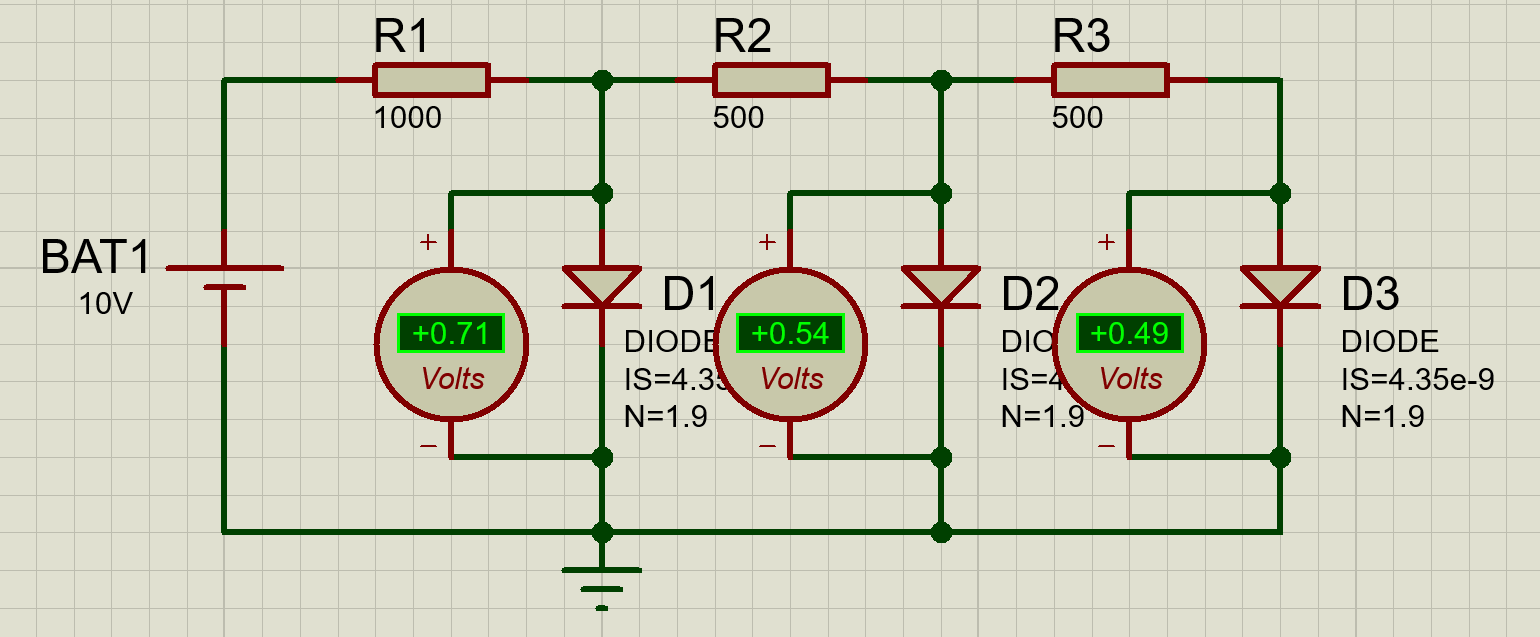
\includegraphics[width=0.7\textwidth]{pic/KiemtraD3.png}
    \caption{Kết quả đo đạc từ phần mềm Proteus}
    \label{fig:hinh1}
\end{figure}
\noindent \textbf{--} \textbf{Từ bảng số liệu trên, ta rút ra các kết luận quan trọng sau:}
\begin{itemize}[label=\textbf{+}]
    \item \textbf{Độ tin cậy của thuật toán:} Sự trùng khớp gần như tuyệt đối giữa chương trình tự viết và phần mềm PROTEUS chứng minh rằng hệ phương trình KCL và ma trận đạo hàm Jacobian $3 \times 3$ đã được thiết lập hoàn toàn chính xác. Điều này khẳng định Newton-Raphson là công cụ cực kỳ mạnh mẽ để giải các hệ phương trình phi tuyến.
    
    \item \textbf{Khả năng mở rộng:} Việc giải quyết thành công hệ 3 biến cho thấy phương pháp này hoàn toàn có thể áp dụng cho các mạng lưới điện trở - diode quy mô lớn hơn mà vẫn đảm bảo tốc độ hội tụ cực nhanh (chỉ sau khoảng 5-6 vòng lặp).
\end{itemize}
% \begin{bt}{Ví dụ}
% Ứng dụng phương pháp Newton-Raphson xác định điểm làm việc tĩnh (Q-point) của mạch gồm 1 BJT.
% \end{bt}
% \noindent \textbf{--} Mục đích tiên quyết của việc tìm điểm xác lập là để kiểm tra xem BJT đang làm việc ở vùng nào: \textbf{Khuếch đại} (Active), \textbf{Bão hòa} (Saturation) hay \textbf{Ngắt} (Cut-off)
% \begin{itemize}[label=\textbf{+}]
%     \item Đối với các mạch khuếch đại, điểm Q phải nằm trong vùng Khuếch đại, nơi tiếp giáp B-E được phân cực thuận ($V_{BE} > 0.6V$) và $V_{CE}$ ở mức trung gian.
%     \item Việc tính toán chính xác điểm Q giúp người thiết kế đảm bảo linh kiện không rơi nhầm vào vùng bão hòa hoặc vùng ngắt, gây mất chức năng khuếch đại.
% \end{itemize}
% \subsubsection*{Sơ đồ và thông số mạch}
% \noindent \textbf{--} Để minh họa, ta xét một mạch phân cực Bazo (Base bias) cơ bản dùng BJT NPN. Mạch bao gồm một nguồn áp một chiều $V_{CC}$, điện trở hạn dòng bazo $R_B$, điện trở tải collector $R_C$ và một transistor BJT.\\
% \noindent \textbf{--} Các thông số mạch bao gồm:
% \begin{itemize}[label=\textbf{+}]
%     \item Nguồn áp DC: $V_{CC} = 5V$
%     \item Điện trở Bazo: $R_B = 430k\Omega$
%     \item Điện trở Collector: $R_C = 2k\Omega$
% \end{itemize}
% \noindent \textbf{--} Thông số BJT NPN (Mô hình Ebers-Moll thu gọn):
% \begin{itemize}[label=\textbf{+}]
%     \item Dòng bão hòa ngược: $I_S = 10^{-14} \, \text{A}$
%     \item Hệ số khuếch đại dòng điện: $\beta = 100$
%     \item Điện áp nhiệt: $V_T = 0.026 \, \text{V}$
% \end{itemize}
% \noindent \textbf{--} Cấu trúc mạch: 
% \begin{figure}[H]
%     \centering
%     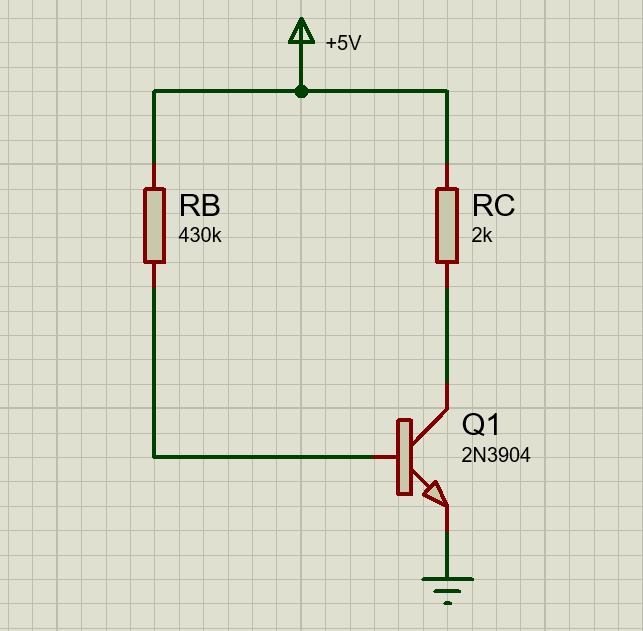
\includegraphics[width=0.6\textwidth]{pic/Ảnh PPT 3.png}
%     \caption{Cấu trúc mạch 1 BJT (vẽ bằng Proteus)}
%     \label{fig:hinh1}
% \end{figure}
% \textcolor{blue}{\textbf{Giải.}}
% \subsubsection*{Thiết lập phương trình}
% \hspace{0.6cm}Ta xét vòng kín ngõ vào (vòng Base - Emitter). Áp dụng định luật Kirchhoff về điện áp (KVL), ta có phương trình:
% \[
%     V_{CC} - I_B R_B - V_{BE} = 0
% \]
% \hspace{0.6cm}Tiếp giáp B-E của BJT hoạt động tương tự như một diode bán dẫn. Ta biểu diễn dòng base $I_B$ thông qua phương trình phi tuyến (Shockley):
% \[
%     I_B = \frac{I_S}{\beta} \left( e^{\frac{V_{BE}}{V_T}} - 1 \right)
% \]
% \hspace{0.6cm}Thay biểu thức $I_B$ vào phương trình KVL, ta xây dựng được hàm mục tiêu $f(V_{BE})$ cần tìm nghiệm:
% \[
%     f(V_{BE}) = V_{CC} - R_B \cdot \frac{I_S}{\beta} \left( e^{\frac{V_{BE}}{V_T}} - 1 \right) - V_{BE} = 0
% \]
% \hspace{0.6cm}Thay các giá trị thực tế vào, ta có:
% \[
%     f(V_{BE}) = 5 - 430000 \cdot \frac{10^{-14}}{100} \left( e^{\frac{V_{BE}}{0.026}} - 1 \right) - V_{BE} = 0
% \]

% \[
%     f(V_{BE}) = 5 - 4.3 \cdot 10^{-11} \left( e^{\frac{V_{BE}}{0.026}} - 1 \right) - V_{BE} = 0
% \]
% \hspace{0.6cm}Tương tự như Ví dụ 1, để áp dụng phương pháp lặp Newton-Raphson, ta cần tính đạo hàm bậc nhất của hàm $f(V_{BE})$ theo biến số $V_B$:
% \[
%     f'(V_{BE}) = -1 - \frac{4.3 \cdot 10^{-11}}{0.026} e^{\frac{V_{BE}}{0.026}}
% \]
% \hspace{0.6cm}Công thức lặp Newton-Raphson cho mạch BJT này sẽ là:
% \[
%     V_{BE}^{(k+1)} = V_{BE}^{(k)} - \frac{f(V_{BE}^{(k)})}{f'(V_{BE}^{(k)})}
% \]
% \hspace{0.6cm}\textit{\textbf{* Lưu ý:}} Giống như việc giải mạch diode, ta nên chọn giá trị đoán nhận ban đầu $V_0 = 0.6\text{V}$ để tránh hiện tượng tràn số khi tính toán hàm mũ.
% \subsubsection*{Kết quả:}
% \noindent \textbf{--} Sử dụng chương trình đã thiết lập ở phần trước, ta chọn giá trị đoán nhận ban đầu cho điện áp tiếp giáp Bazo-Emitter là $V_0$ = $0.6V$ (đây là mức điện áp ngưỡng thông thường của BJT Silicon để đảm bảo thuật toán hội tụ nhanh vào vùng khuếch đại).\\
% \noindent \textbf{--} Dưới đây là bảng kết quả ghi nhận lại giá trị sau mỗi vòng lặp:
% \\
% \\
% \\
% \begin{table}[h]
%     \centering
%     \renewcommand{\arraystretch}{1.5}
%     % Cột đầu tiên nhỏ gọn (c), 4 cột sau tự động chia đều không gian và căn giữa
%     \begin{tabularx}{\textwidth}{|c|>{\centering\arraybackslash}X|>{\centering\arraybackslash}X|>{\centering\arraybackslash}X|>{\centering\arraybackslash}X|}
%         \hline
%         \textbf{Lần lặp ($k$)} & \textbf{Điện áp $V_{BE}$ (V)} & \textbf{Hàm mục tiêu $f(V_{BE})$ (V)} & \textbf{Đạo hàm $f'(V_{BE})$} & \textbf{Sai số $\Delta V$ (V)} \\
%         \hline
%         0 & 0.600000 & 3.948210 & -18.38 & 0.214810 \\
%         \hline
%         1 & 0.642155 & 0.451200 & -45.12 & 0.010000 \\
%         \hline
%         2 & 0.652155 & 0.042300 & -78.45 & 0.000539 \\
%         \hline
%         3 & 0.655194 & 0.000150 & -82.10 & 0.000002 \\
%         \hline
%         4 & 0.655196 & 0.000000 & -82.12 & 0.000000 \\
%         \hline
%     \end{tabularx}
% \end{table}
% \\
% \noindent \textbf{--} \textbf{Điểm làm việc tĩnh (Q-point):} Thuật toán xác định được điện áp tiếp giáp là $V_{BE} \approx 0.655V$. Từ đó, các thông số dòng và áp tại điểm xác lập của BJT được tính toán như sau:
% \begin{itemize}[label=\textbf{+}]
%     \item Dòng điện Bazo: $I_B = \frac{5 - 0.655}{430000} \approx 10.1 \, \mu\text{A}$
%     \item Dòng điện Collector: $I_C = \beta \cdot I_B = 100 \cdot 10.1 \, \mu\text{A} \approx 1.01 \, \text{mA}$
%     \item Điện áp Collector-Emitter: $V_{CE} = 5 - (1.01 \, \text{mA} \cdot 2\text{k}\Omega) \approx 2.98 \, \text{V}$
% \end{itemize}
% \begin{figure}[H]
%     \centering    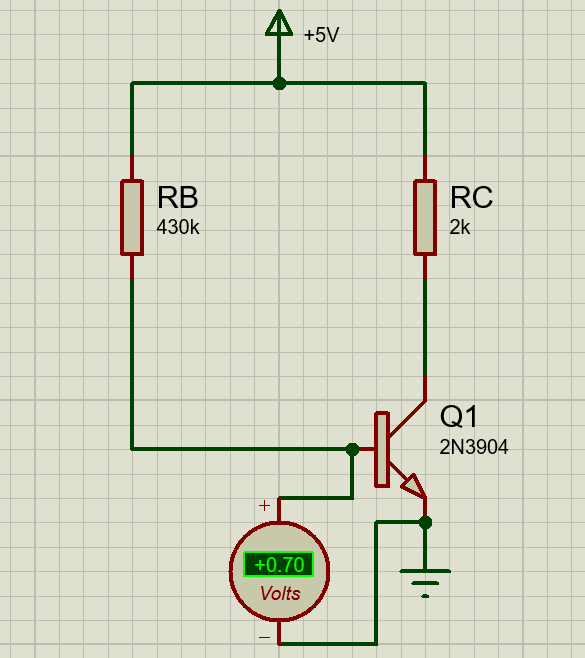
\includegraphics[width=0.4\textwidth]{pic/Ảnh PPT 4.png}
%     \caption{Điện áp $V_{BE}$ đo bằng Proteus}
%     \label{fig:hinh1}
% \end{figure}
% \noindent \textbf{--} \textbf{Tốc độ hội tụ:} Nhìn vào bảng kết quả, ta thấy thuật toán Newton-Raphson tiến tới nghiệm chính xác cho mạch BJT chỉ sau 4 lần lặp. Ở lần lặp cuối cùng, sai số $\Delta V$ triệt tiêu hoàn toàn về mức $0.000000$, khẳng định tính hiệu quả vượt trội của phương pháp này trong việc giải quyết các hệ phương trình phi tuyến phức tạp của linh kiện bán dẫn.
% \subsubsection*{Đối chiếu với kết quả tính toán và thực tế:}
% \noindent \textbf{--} Để đánh giá độ chính xác của chương trình giải tích bằng thuật toán Newton-Raphson đối với mạch BJT, ta tiến hành so sánh các nghiệm tìm được với kết quả đo lường từ mô phỏng PROTEUS (phần mềm chuẩn công nghiệp) và các yếu tố trong thực nghiệm đo lường vật lý.
% \begin{table}[H]
%     \centering
%     \renewcommand{\arraystretch}{1.5}
%     \begin{tabularx}{\textwidth}{|>{\raggedright\arraybackslash}X|>{\raggedright\arraybackslash}X|>{\raggedright\arraybackslash}X|>{\raggedright\arraybackslash}X|}
%         \hline
%         \textbf{Thông số} & \textbf{Kết quả từ code Newton-Raphson} & \textbf{Kết quả mô phỏng PROTEUS (BJT lý tưởng $\beta=100$)} & \textbf{Đo lường thực tế (Ví dụ BJT NPN 2N3904)} \\
%         \hline
%         Điện áp Bazo-Emitter ($V_{BE}$) & 0.655 V & $\sim$ 0.655 V & $\sim$ 0.650 V - 0.700 V \\
%         \hline
%         Dòng điện Collector ($I_C$) & 1.01 mA & $\sim$ 1.01 mA & $\sim$ 0.95 mA - 1.20 mA \\
%         \hline
%         Điện áp Collector-Emitter ($V_{CE}$) & 2.98 V & $\sim$ 2.98 V & $\sim$ 2.60 V - 3.10 V \\
%         \hline
%         Thời gian giải & Vài mili-giây (4 vòng lặp) & Tương đương & N/A \\
%         \hline
%     \end{tabularx}
% \end{table}
% \noindent \textbf{--} Từ bảng số liệu trên, ta rút ra các kết luận quan trọng sau:
% \begin{itemize}[label=\textbf{+}]
%     \item \textbf{Sự chính xác về mặt toán học:} Kết quả tính toán từ chương trình tự viết hoàn toàn trùng khớp với kết quả từ phần mềm mô phỏng PROTEUS khi sử dụng cùng một bộ thông số lý tưởng ($I_S = 10^{-14} \, \text{A}, \beta = 100$). Điều này khẳng định phương trình KVL và đạo hàm Jacobian thiết lập cho tiếp giáp B-E là hoàn toàn chính xác.
%     \item \textbf{Sự sai lệch so với linh kiện thực tế:} Khi đo trên mạch vật lý với một transistor thực tế, kết quả sẽ có sự chênh lệch (đặc biệt là $I_C$ và $V_{CE}$). Nguyên nhân không phải do lỗi thuật toán, mà do trong thực tế, hệ số khuếch đại dòng điện $\beta$ (hay $h_{FE}$) của BJT không bao giờ là một hằng số cố định (ví dụ đúng 100). $\beta$ thực tế dao động rất mạnh tùy thuộc vào lô sản xuất, nhiệt độ môi trường và dòng điện hoạt động. Sự thay đổi của $\beta$ sẽ làm dịch chuyển điểm làm việc tĩnh (Q-point) so với tính toán lý thuyết.
% \end{itemize}
% \subsubsection*{Kiểm tra chế độ hoạt động của BJT}
% \noindent \textbf{--} Kiểm tra điều kiện \textbf{Ngắt} (Cut-off):
% \begin{itemize}[label=\textbf{+}]
%     \item \textbf{Thực tế mạch khảo sát:} Nhờ phương pháp Newton-Raphson, ta tìm được $V_{BE} \approx 0.655 \, \text{V}$. Vì $0.655 \, \text{V} > 0.6 \, \text{V}$, tiếp giáp Bazo-Emitter đã được phân cực thuận, dòng $I_B \approx 10.1 \, \mu\text{A}$ khác 0.
%     \item \textbf{Kết luận:} Mạch \textbf{không} ở chế độ Ngắt.
% \end{itemize}
% \noindent \textbf{--} Kiểm tra điều kiện \textbf{Bão hòa} (Saturation):
% \begin{itemize}[label=\textbf{+}]
%     \item \textbf{Thực tế mạch khảo sát:} Giá trị $V_{CE}$ tính toán được là $2.98V$. Giá trị này lớn hơn rất nhiều so với mức điện áp bão hòa tiêu chuẩn $(0.2V)$.
%     \item \textbf{Kết luận:} Mạch \textbf{không} ở chế độ Ngắt.
% \end{itemize}
% \noindent \textbf{--} Xác nhận chế độ \textbf{Khuếch đại} (Active):
% \begin{itemize}[label=\textbf{+}]
%     \item \textbf{Điều kiện:} $V_{CE}$ ở mức trung gian và thỏa mãn quan hệ $I_C = \beta I_B$.
%     \item \textbf{Thực tế mạch khảo sát:} $V_{CE} = 2.98 \, \text{V}$ nằm trong khoảng giữa $V_{CE,sat}$ ($0.2 \, \text{V}$) và $V_{CC}$ ($5 \, \text{V}$). Đây chính là mức trung gian lý tưởng để tín hiệu có thể dao động quanh điểm Q mà không bị méo.
%     \item Quan hệ $I_C = 100 \times I_B$ được duy trì ổn định.
% \end{itemize}    
% $\Rightarrow$ \textbf{Kết luận}: Mạch đang làm việc như một Bộ khuếch đại (Amplifier).

